


\section{Proposta}

\subsection{Proposta}



\begin{frame}\frametitle{Trabalho anterior}
\begin{columns}
	\begin{column}{5cm}
	\begin{itemize}
		\item Ao final de POC I, foi poss�vel gerar terrenos na CPU.
		\item O terreno era dividido em quadrados, que eram gerados proceduralmente a medida que era necess�rio.
	\end{itemize}
	\vspace{3cm} 
	\end{column}
	\begin{column}{5cm}
	\begin{overprint}
		\includegraphics<1>[width=1.0\linewidth]{img/poc1}
	\end{overprint}
	\end{column}
\end{columns}
\end{frame}


\begin{frame}\frametitle{Proposta}
\begin{itemize}
	\item O objetivo deste trabalho � expandir oque foi implementado em POC I, dessa vez para terrenos maiores.
	\item Para isso, buscou-se transferir a gera��o dos terrenos da \texttt{CPU} para a \texttt{GPU} (placas de v�deo).
\end{itemize}
\end{frame}


\subsection{Gera��o procedural dos terrenos}

\begin{frame}\frametitle{Ru�do de Perlin}
\begin{columns}
	\begin{column}{5cm}
	\begin{itemize}
		\item O ru�do � usado para simular estruturas naturais, como n�vens, texturas de �rvores, e terrenos.
	\end{itemize}
	\vspace{3cm} 
	\end{column}
	\begin{column}{5cm}
	\begin{overprint}
		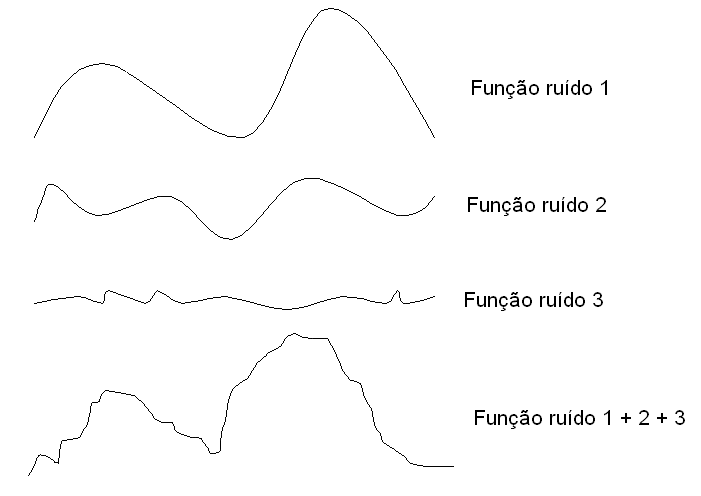
\includegraphics[width=1.0\linewidth]{img/perlin}
	\end{overprint}
	\end{column}
\end{columns}
\end{frame}


\begin{frame}\frametitle{Gera��o na GPU}
\begin{columns}
	\begin{column}{5cm}
	\begin{itemize}
		\item A natureza facilmente paraleliz�vel das aplica��es gr�ficas fez com que as GPUs fossem desenvolvidas com um n�mero muito maior de unidades de processamento do que as CPUs.
		\item Como o terreno vai ser gerado (e desenhado) na GPU, n�o haver� perda na transfer�ncia de dados do terreno entre CPU e GPU.
	\end{itemize}
	\vspace{3cm} 
	\end{column}
	\begin{column}{5cm}
	\begin{overprint}
		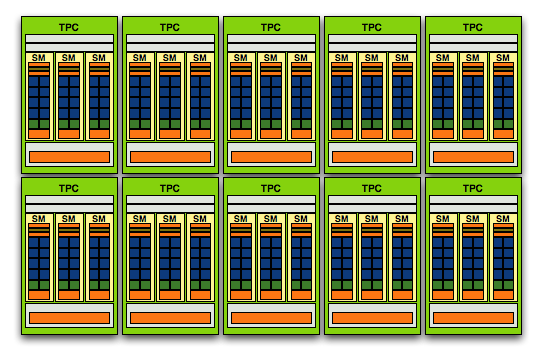
\includegraphics[width=1.0\linewidth]{img/gpu}
	\end{overprint}
	\end{column}
\end{columns}
\end{frame}

\begin{frame}\frametitle{Gera��o na GPU}
\begin{columns}
	\begin{column}{5cm}
	\begin{itemize}
		\item A gera��o ser� feita atrav�s de conjuntos de instru��es (shaders) executados na GPU.
		\item O \emph{pipeline} gr�fico das GPUs executa dois tipos de shaders:
		\begin{itemize}
			\item \tiny Vertex shader: executado para cada v�rtice da cena.
			\item \tiny Fragment shader: executado para cada fragmento dos pol�gonos (a sa�da do shader � uma cor, salva em uma textura).
		\end{itemize}
	\end{itemize}
	%\vspace{3cm} 
	\end{column}
	\begin{column}{7cm}
	\begin{overprint}
		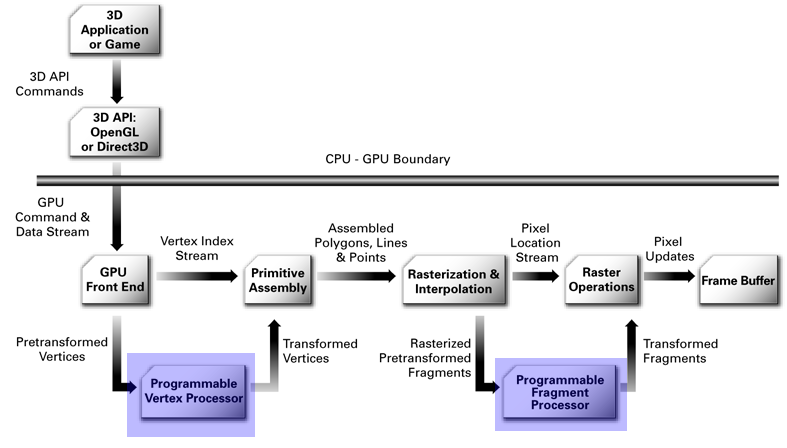
\includegraphics[width=1.0\linewidth]{img/pipeline}
	\end{overprint}
	\end{column}
\end{columns}
\end{frame}



\begin{frame}\frametitle{Gera��o na GPU}
\begin{columns}
	\begin{column}{7cm}
	\begin{itemize}
		\item Fragment shader: calcular o novo terreno procedural e salva o resultado em uma textura.
		\item Vertex shader: ap�s o calculo do terreno, ir� consultar oque foi gerado, e ajustar a altura dos v�rtices do terreno.
		\item Para evitar efeitos indesej�veis do terreno sendo criado a medida que o usu�rio se move, o terreno � criado em passos, cada um sendo exibido quando est� pronto.
	\end{itemize}
	\vspace{3cm} 
	\end{column}
	\begin{column}{5cm}
	\begin{overprint}
		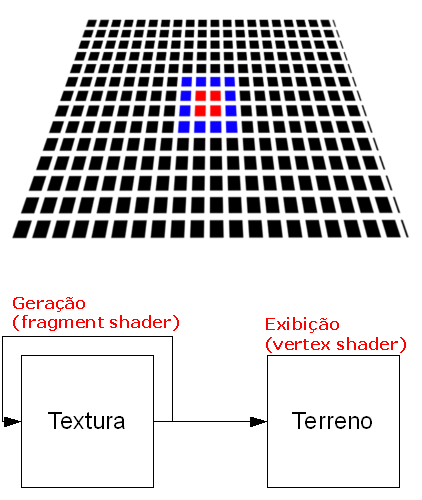
\includegraphics[width=1.0\linewidth]{img/geracao}
	\end{overprint}
	\end{column}
\end{columns}
\end{frame}






